\documentclass{standalone}
\usepackage{tikz,tikz-3dplot}
\usetikzlibrary{perspective,patterns}
\usetikzlibrary{calc,fadings,decorations.pathreplacing}
\usetikzlibrary{shapes,fit}
\usetikzlibrary{hobby}
\usetikzlibrary{arrows.meta}
\begin{document}
\tikzset{illustration/.style={very thin}}
\tikzset{dimension/.style={very thin,lightgray}}
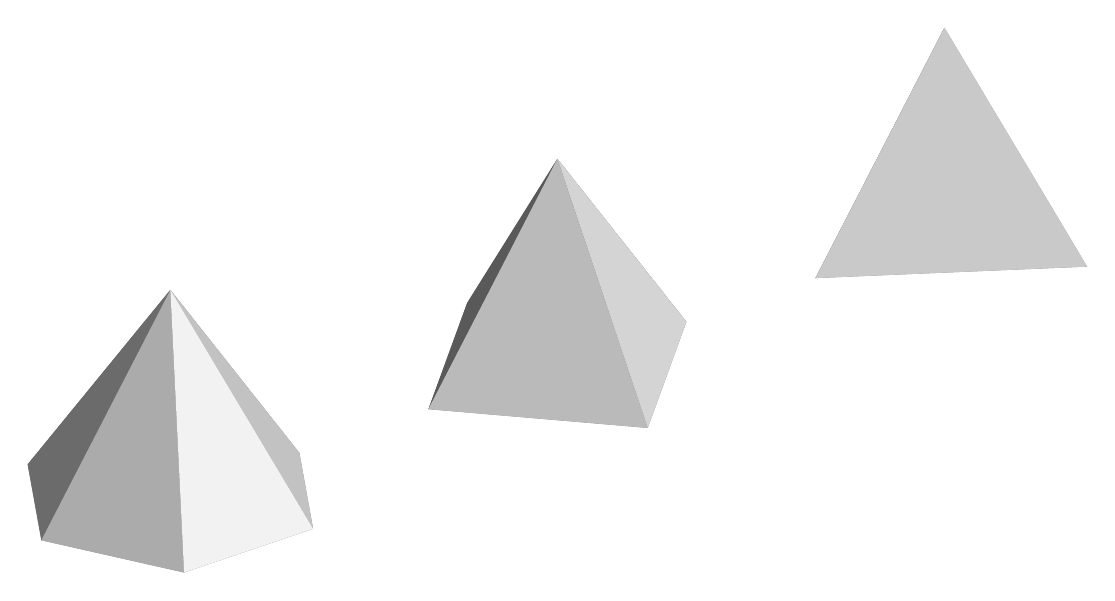
\begin{tikzpicture}[3d view={145.0079798014413}{28.941784084694106},fill=gray]
\fill (-1.0,-1.7321)--(-1.0,1.7321)--(2.0,0.0)--cycle;
\fill (6.0,-2.0)--(4.0,0)--(6.0,2.0)--(8.0,0.0)--cycle;
\fill (13.0,-1.7321)--(11.0,-1.7321)--(10.0,0)--(11.0,1.7321)--(13.0,1.7321)--(14.0,0.0)--cycle;
\fill[white!60!black] (0,0,3)--(-1.0,1.7321,0.0)--(-1.0,-1.7321,0.0)--cycle;
\fill[white!28!black] (0,0,3)--(-1.0,-1.7321,0.0)--(2.0,0.0,0.0)--cycle;
\fill[white!79!black] (0,0,3)--(2.0,0.0,0.0)--(-1.0,1.7321,0.0)--cycle;
\fill[white!42!black] (6,0,3)--(4.0,0,0.0)--(6.0,-2.0,0.0)--cycle;
\fill[white!35!black] (6,0,3)--(6.0,-2.0,0.0)--(8.0,0.0,0.0)--cycle;
\fill[white!83!black] (6,0,3)--(6.0,2.0,0.0)--(4.0,0,0.0)--cycle;
\fill[white!73!black] (6,0,3)--(8.0,0.0,0.0)--(6.0,2.0,0.0)--cycle;
\fill[white!33!black] (12,0,3)--(11.0,-1.7321,0.0)--(13.0,-1.7321,0.0)--cycle;
\fill[white!49!black] (12,0,3)--(10.0,0,0.0)--(11.0,-1.7321,0.0)--cycle;
\fill[white!42!black] (12,0,3)--(13.0,-1.7321,0.0)--(14.0,0.0,0.0)--cycle;
\fill[white!76!black] (12,0,3)--(11.0,1.7321,0.0)--(10.0,0,0.0)--cycle;
\fill[white!67!black] (12,0,3)--(14.0,0.0,0.0)--(13.0,1.7321,0.0)--cycle;
\fill[white!95!black] (12,0,3)--(13.0,1.7321,0.0)--(11.0,1.7321,0.0)--cycle;
\end{tikzpicture}
\end{document}
